\documentclass[manuscript,screen,review]{acmart}
\usepackage[brazil]{babel}
\usepackage[utf8]{inputenc}

\AtBeginDocument{%
  \providecommand\BibTeX{{%
    \normalfont B\kern-0.5em{\scshape i\kern-0.25em b}\kern-0.8em\TeX}}}

\setcopyright{acmcopyright}
\copyrightyear{2023}
\acmYear{2023}
\acmDOI{XXXXXXX.XXXXXXX}

\acmConference[UFSJ '23]{Universidade Federal de São João del-Rei}{Junho 30--06, 2023}{São João del-Rei, MG}

\settopmatter{printacmref=false}

\begin{document}

\title{Identificando URLs Maliciosas: Uma Abordagem Puramente Léxica}

\author{Julio Rodrigues}
\email{julio.csr.271@aluno.ufsj.edu.br}
\affiliation{%
  \institution{Universidade Federal de São João del-Rei}
  \city{São João del-Rei}
  \state{Minas Gerais}
  \country{Brasil}
  \postcode{36.301-360}
}

\renewcommand{\shortauthors}{Rodrigues, J.}

\begin{abstract}
Neste trabalho, apresentamos um método eficaz de detecção de URLs maliciosas de vários tipos baseando-se em aprendizado de máquina. Com o intuito de evitar quaisquer necessidades de acessos à tais URLs para extração de informações, somente foram utilizadas características pertencentes ao escopo léxico da URL. As análises foram executadas com bases de dados já consolidadas como as disponíveis no Kaggle e PhishTank, obtendo resultados competitivos com trabalhos relacionados que utilizam de características relacionadas à rede ou conteúdo das URLs.\looseness=-1
\end{abstract}

\keywords{feature construction, características léxicas, detecção de URLs, balanceamento de classes}

\received[Recebido]{30 Junho 2023}
% \received[Revisado]{3 Agosto 2023}
% \received[Aceito]{10 Agosto 2023}

\maketitle

\section{Introdução}

De modo geral, o elo mais fraco quando se trata de segurança na internet é o ser humano, mais especificamente o usuário. URLs são vias rápidas e diretas para possibilitar ações maliciosas na internet, bastando no máximo alguns cliques para efetivação de um ataque cibernético. Por isto, o potencial de infecção por este meio é extremamente alto, embora a efetividade de parte destes ataques dependa de características adicionais da URL e de técnicas de camuflagem utilizadas.

Em 2019, segundo relatório\footnotemark \hspace{0.1cm}da Abranet, o Brasil estava no top 15 entre os países com o maior número de vítimas de ataques cibernéticos com URLs maliciosas. Atualmente, estas estatísticas possivelmente podem apresentar-se bem piores, devido ao período transcorrido da pandemia de \emph{Covid-19}, cuja uma das consequências foi a elevação do uso de tecnologias da informação de modo geral. É um campo em que existe uma constante evolução dos dois lados conflitantes. O lado de combate, aprimorando as técnicas para detecção, e o lado de ataque, evoluindo as técnicas de camuflagem das URLs.

\footnotetext[1]{\scriptsize Disponível em: \url{https://www.abranet.org.br/Noticias/Relatorio-aponta-que-cada-URL-maliciosa-no-Brasil-afeta-18-usuarios-2585.html?UserActiveTemplate=site}}

Atualmente, existem duas estratégias populares eficazes utilizadas na detecção de URLs maliciosas. A primeira delas são os serviços de \emph{blacklist}. Tais serviços consistem no armazenamento de URLs reportadas e rotuladas como maliciosas, oferecendo um serviço de consulta para verificação de URLS suspeitas que se encontram no banco de dados. Embora este serviço seja eficaz a médio e longo prazo, este é em grande parte das vezes incapaz de verificar ou catalogar URLs maliciosas recém-formadas.

A segunda abordagem consiste na construção de modelos de aprendizado de máquina para classificação de URLs. A utilização destes tipos de métodos geralmente apresenta maior complexidade geral em relação aos serviços de \emph{blacklist}. No entanto, em caso de sucesso com um modelo bem construído, este pode apresentar eficácia a curto, médio e longo prazo, capaz de classificar grande parte das URLs com precisão.

A organização deste artigo apresenta-se na seguinte forma: a Seção \ref{sec:2} apresenta alguns dos trabalhos relacionados; na Seção \ref{sec:3} é descrita a metodologia de desenvolvimento empregada; a Seção \ref{sec:4} apresenta uma análise sobre os resultados obtidos; a Seção \ref{sec:5} discute as principais conclusões deste trabalho e apresenta uma série de questões a serem consideradas em possíveis trabalhos futuros. 

\section{Trabalhos Relacionados} \label{sec:2}

Ayres et al. \cite{sbrc} propõem um modelo de classificação binária de URLs de \emph{phishing} direcionadas a brasileiros. Os autores extraíram um conjunto de 117 características das URLs, incluindo as de escopo léxico e de rede. Destas 117 características, as três que possuem maior poder preditivo estão relacionadas à rede, exigindo o acesso às URLs para que tais informações sejam coletadas. Os resultados apresentados revelam bom desempenho de classificadores clássicos, com \emph{F1 Score} média de 95,85\% entre KNN, SVM e J48 (Árvore de Decisão).

Saleem Raja et al. \cite{SALEEMRAJA2021163} propõem um estudo baseado somente na construção de atributos léxicos para formular um classificador de URLs multiclasse. Ao todo, foram extraídos 27 características da base de dados, embora somente as 20 com maior poder preditivo foram utilizadas no modelo final. Tal modelo alcançou \emph{F1 Score} de 99\% com o algoritmo \emph{ensemble} random forest, embora não tenham utilizado quaisquer técnicas de validação cruzada.

Vazhayil et al. \cite{8494159} executam um comparativo entre métodos de aprendizado profundo e aprendizado de máquina para classificação binária de URLs de \emph{phishing}. Os resultados apresentados revelam que a combinação de redes neurais (CNN e LSTM) são capazes de prover um modelo com \emph{F1 Score} de até 98\%.

Aljabri et al. \cite{10.1155/2022/3241216} também seguem uma abordagem semelhante, utilizando modelos de aprendizado de máquina e aprendizado profundo para classificação binária de URLs. No entanto, é extraído um conjunto de características baseadas não apenas no escopo léxico da URL, mas também de aspectos relacionados à rede e conteúdo. O modelo construído alcançou \emph{F1 Score} de 96\% com um dos classificadores mais simples do aprendizado de máquina supervisionado: o Naive Bayes.

Por fim, Ateeq e Moreb \cite{9493481} trabalharam no desenvolvimento de um método para classificação multiclasse, utilizando um método de aprendizado profundo. Foram extraídas um total de apenas 8 características das URLs, todas no escopo léxico, estas que alimentaram um rede neural \emph{feedforward} com múltiplas camadas ocultas. Como resultado final, observou-se uma \emph{F1 Score} de 98,48\%. 

\section{Metodologia} \label{sec:3}

Nesta seção, apresentamos em detalhes o processo de desenvolvimento e decisões cruciais tomadas na concepção de um método eficaz para classificação de URLs, baseado em aprendizado de máquina. É importante citar de antemão, que todo o desenvolvimento deste trabalho foi realizado utilizando a linguagem Python\footnotemark \hspace{0.1cm}em conjunto com a biblioteca de aprendizado de máquina de código aberto \emph{scikit-learn\footnotemark}. A implementação encontra-se disponível publicamente em \url{https://github.com/juliorodrigues07/url_detection}.

\footnotetext[2]{\scriptsize Mais informações em: \url{https://www.python.org/}}
\footnotetext[3]{\scriptsize Mais informações em: \url{https://scikit-learn.org/stable/}}

\subsection{Extração de Características}

No processo de extração de informações das URLs com alto poder preditivo, decidimos utilizar uma abordagem puramente léxica. Portanto, tal processo ocorre somente no escopo da estrutura da URL. O principal motivo por detrás desta abordagem, é de que a extração da maioria das características relacionadas a conteúdo ou rede de URLs abordada em vários trabalhos relacionados, exige o acesso às mesmas para coleta. Idealmente, não deveria haver necessidade de acessá-las. Pelo contrário, desejamos saber a natureza de uma URL sem riscos de vulnerabilidade aos ataques cibernéticos.

Neste trabalho, extraímos 7 características por meio de simples análises estatísticas das bases de dados, enquanto outras 14 características foram extraídas com base na análise de trabalhos relacionados. Novamente, todas estas 21 características foram extraídas considerando somente o escopo léxico das URLs.

Entre as características mais simples extraídas, se encontram a contabilização de símbolos (\emph{tokens}) diversos presentes nas URLs. É possível encontrar discrepâncias interessantes em relação a estas quantidades, como por exemplo, a quantidade de símbolos "=" \hspace{0.1cm}presentes nas URLs. URLs do tipo \emph{defacement} apresentam, em média, uma quantidade 11 vezes maior deste símbolo em relação a outros tipos de URL na base de dados coletada.

Além da contagem de símbolos, também foram extraídas características relacionadas à medição de segmentos das URLs. Neste ponto, são consideradas métricas como o comprimento em número de caracteres das URLS e tamanho do diretório como características com potencial de distinguir instâncias maliciosas de seguras.

\subsection{Seleção de Características}

\vspace*{-1cm}
\begin{figure}[ht]
    \centering
    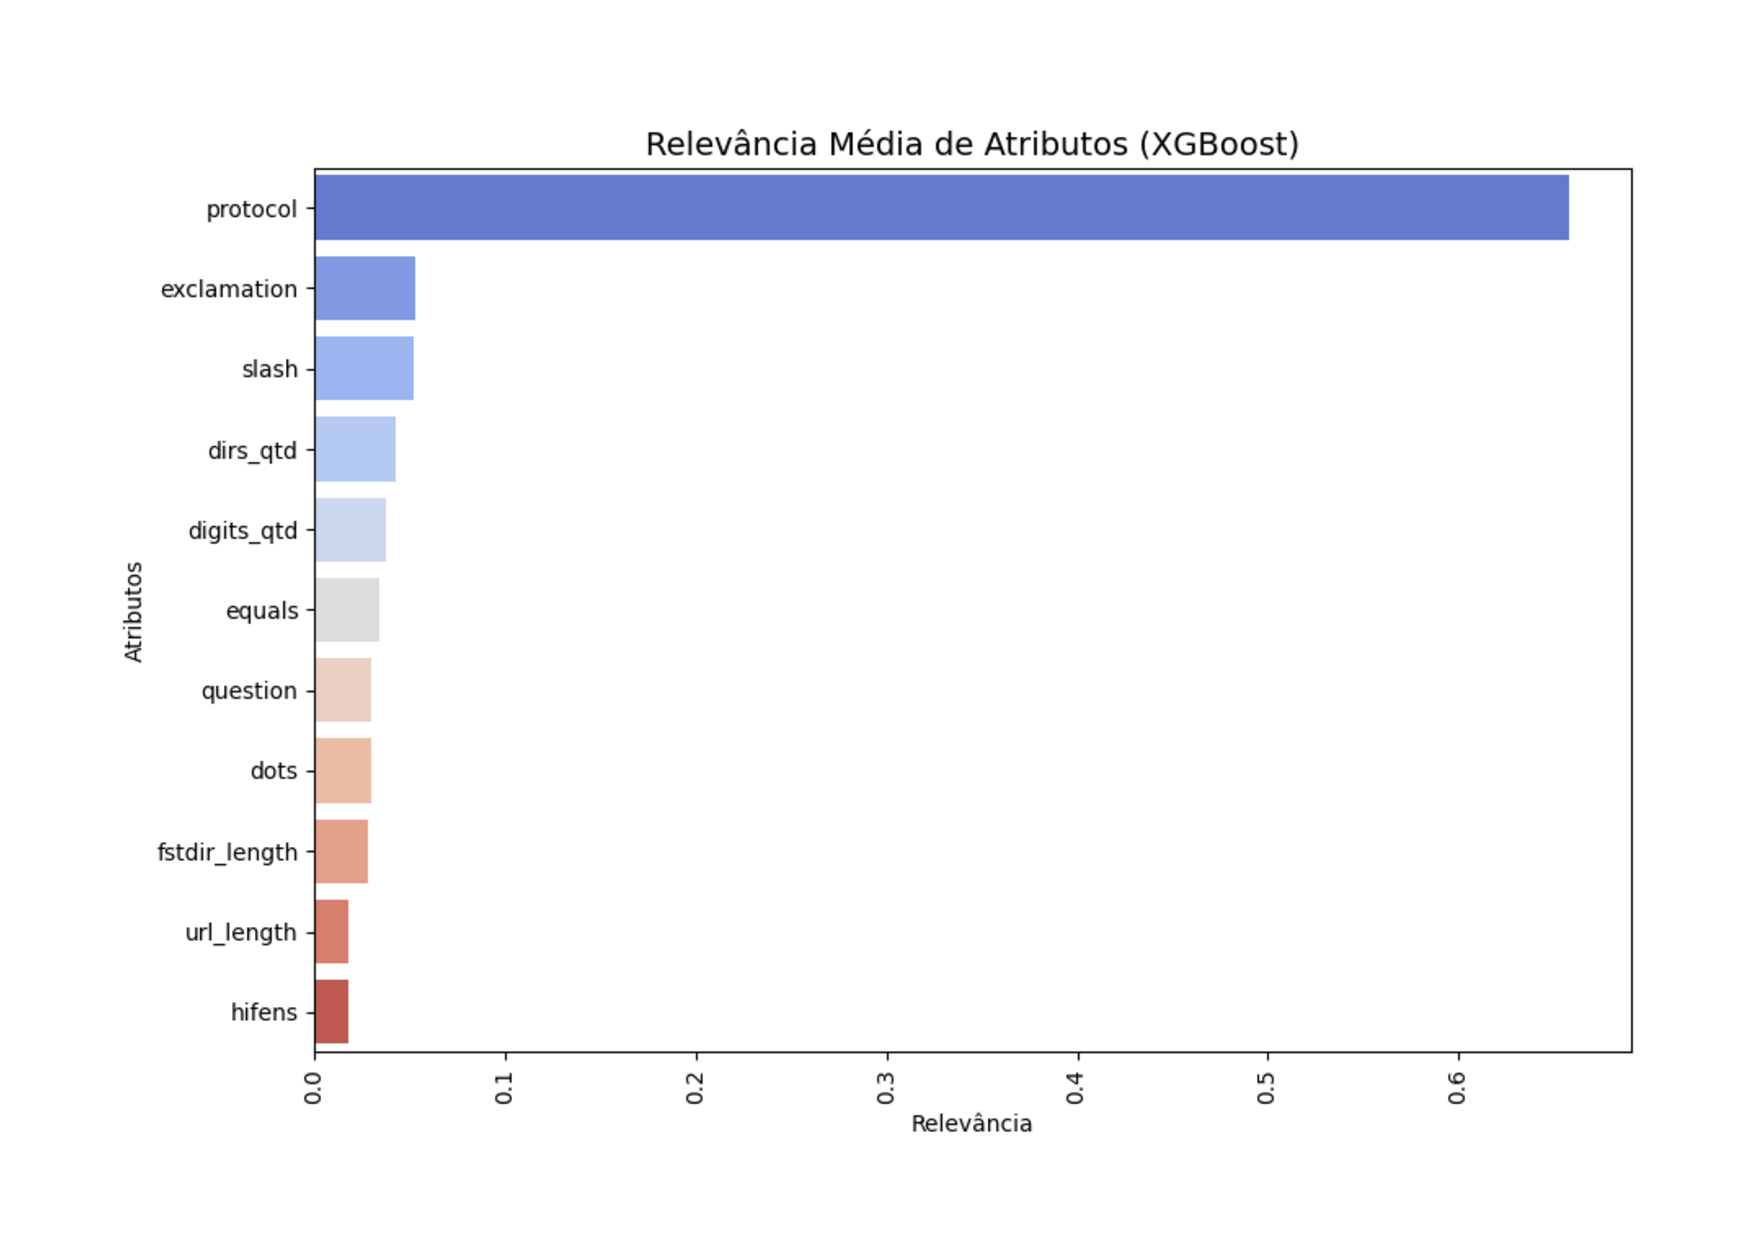
\includegraphics[width=1\textwidth]{pic/attr.pdf}
    \vspace*{-1cm}
    \caption{Poder preditivo das 11 características}
    \label{fig:exampleFig1}
\end{figure}

Concluído o processo de extração de características, iniciou-se a etapa de análise da relevância de cada uma destas. Para realizar este tipo de análise, utilizamos uma estratégia de eliminação recursiva de características com validação cruzada. Em outras palavras, utilizamos uma estratégia \emph{bottom-up}, dividindo a base em cinco partes a cada eliminação de característica com menor relevância na classificação, obtendo 11 características de maior poder preditivo ao final do processamento.

Este processo é executado até que se encontre uma quantidade ótima de características, ou seja, o total de características eliminadas provocam pouco, ou nenhum impacto no desempenho do modelo. Na Figura \ref{fig:exampleFig1}, podemos observar o resultado da seleção de características utilizando o algoritmo XGBoost \cite{10.1145/2939672.2939785} como base. É evidente a discrepância do poder preditivo do protocolo de comunicação utilizado pelas URLs com o restante dos atributos. Este comportamento deve-se a padrões muito bem definidos encontrados na base de dados, com a totalidade URLs de \emph{defacement} utilizando o protocolo HTTP, e URLs de \emph{phishing} e \emph{malware} concentrando-se no protocolo HTTPS.

\subsection{Base de Dados e Balanceamento}

Para a construção do modelo de aprendizado de máquina supervisionado, utilizamos URLs presentes em duas bases de dados:

\begin{itemize}
    \setlength{\itemsep}{10pt}
    \item \textbf{Kaggle}\footnotemark: Base de dados composta por 651.191 URLs coletadas de diversas fontes, distribuídas entre quatro classes;
    \item \textbf{PhishTank}\footnotemark: Base de dados composta exclusivamente por URLs de \emph{phishing}. Foram coletadas 105.905 instâncias. 
\end{itemize}

\footnotetext[4]{\scriptsize Disponível em: \url{https://www.kaggle.com/datasets/sid321axn/malicious-urls-dataset}}
\footnotetext[5]{\scriptsize Disponível em: \url{https://phishtank.org/phish_archive.php}}

Após a aplicação do processo de união e remoção de instâncias duplicadas das bases de dados, tornou-se evidente o desbalanceamento de classes (Figura \ref{fig:exampleFig2}). Tal aspecto tornou necessária a adoção de técnicas de balanceamento precedendo a etapa de treinamento dos classificadores.

Neste ponto, optamos por uma abordagem híbrida em relação à aplicação das técnicas de balanceamento na base de dados. O caminho mais simples seria à aplicação indiscriminada de \emph{oversampling} aleatório, duplicando instâncias das classes minoritárias, sem necessariamente agregar informação útil para os processos de treinamento e classificação. Além disso, o volume de dados duplicaria, elevando significativamente o custo computacional para treinamento dos modelos.

Todavia, após testes iniciais com método \emph{hold-out}, verificou-se que os valores da métrica \emph{F1 Score} apresentaram-se próximos para URLs de classes \emph{benign}, \emph{phishing} e \emph{defacement}. Este resultado preliminar indicou uma potencial aplicação de \emph{undersampling} aleatório em instâncias da classe majoritária (\emph{benign}). Esta técnica foi de fato executada posteriormente, reduzindo o número de URLs seguras na base de dados de 428.081 para 200.000 instâncias. Com isto, concedeu-se margem para evitar perda de informação no caso de remoção de grandes quantidades de URLs não redundantes.

Nesta etapa, equiparamos o número de instâncias de URLs seguras e de \emph{phishing}, por meio de \emph{undersampling} aleatório e raspagem de dados na base da PhishTank, respectivamente. Restou-se então, o nivelamento das URLs de \emph{defacement} e \emph{malware}. Embora houvesse a tentativa de raspagem de dados como no caso das URLs de \emph{phishing}, não encontramos bases de dados suficientemente grandes para suprir o déficit de tais instâncias.

No entanto, decidimos por aplicar uma técnica de balanceamento baseada em sobreamostragem minoritária sintética: SMOTE \cite{DBLP:journals/corr/abs-1106-1813}. Em outras palavras, foram criadas diversas instâncias sintéticas das classes \emph{defacement} e \emph{malware} com base em URLs existentes dos tipos na base de dados.

Por fim, obtemos uma base de dados totalmente balanceada, com 800 mil URLs (200 mil instâncias de cada classe) e 11 características. Desta etapa em diante, podemos prosseguir com a escolha dos algoritmos de aprendizado de máquina, formulação e avaliação dos modelos.

\begin{figure}[H]
    \centering
    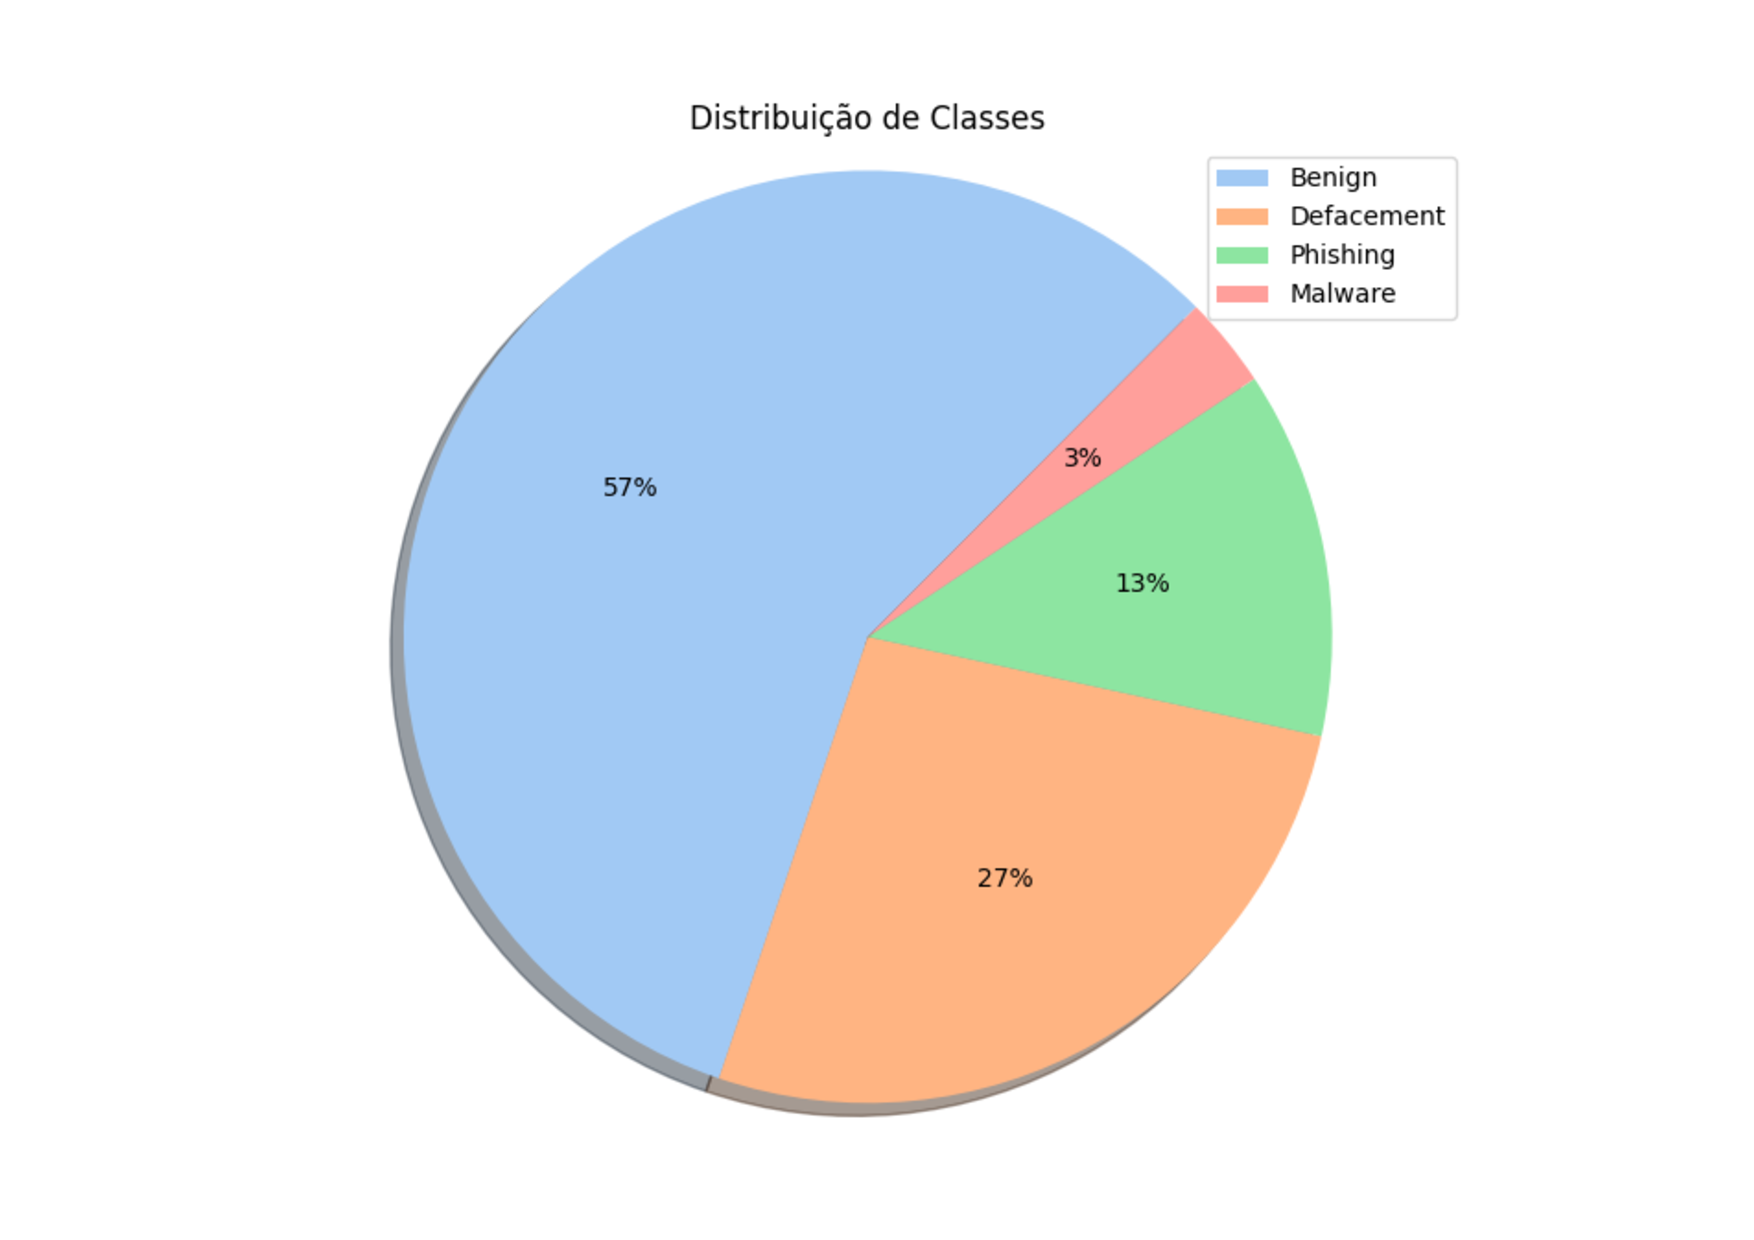
\includegraphics[width=1\textwidth]{pic/class.pdf}
    \caption{Proporções das classes na base de dados}
    \label{fig:exampleFig2}
\end{figure}

\subsection{Seleção de Classificadores}

Para construção dos modelos de aprendizado de máquina supervisionado, selecionamos um conjunto com três classificadores. O primeiro deles é o XGBoost, caracterizado como um método \emph{ensemble}, este utiliza um conjunto de vários classificadores com a técnica de \emph{boosting}, calibrando e reforçando os classificadores a cada iteração. Os dois algoritmos restantes correspondem a métodos considerados clássicos da literatura, a regressão logística e o KNN \cite{fix1951discriminatory}.

O principal motivo por trás da escolha de tais algoritmos, é a oportunidade de observar e comparar o desempenho de um classificador mais recente e sofisticado (XGBoost) com algoritmos mais antigos e clássicos (e.g, KNN). Neste ponto, podemos levantar algumas questões como por exemplo, a relação de desempenho do classificador com o custo computacional associado para treinamento. Outra hipótese a ser levantada é a influência do processo KDD no desempenho final dos classificadores, ou seja, se existe diferença real entre os classificadores com uma base de dados bem polida.

\subsection{Avaliação dos Modelos}

Na avaliação dos resultados, utilizamos a técnica de validação cruzada com 10 partes (\emph{10-fold}). Executada toda a bateria de testes, obtemos a média e o desvio padrão da métrica \emph{Macro F1} para analisar o desempenho de cada algoritmo.

Por fim, também realizamos o ajuste fino dos hiperparâmetros para cada algoritmo com o experimento \emph{tripartite} com 5 partes (\emph{5-fold}), e um teste estatístico para cada par de algoritmos (Teste t de Dupla Cauda). Este teste é executado para determinar se os modelos são estatisticamente similares ou distintos com determinado nível de confiança. 

\section{Resultados} \label{sec:4}

Os resultados obtidos com cada algoritmo com validação cruzada com 10 partes, após o ajuste fino dos hiperparâmetros, são sumarizados na Tabela \ref{tab:exampleTab1}. Inicialmente, podemos observar um desempenho bom e similar entre os algoritmos XGBoost e KNN, que será discutido mais adiante com o teste estatístico. O desvio padrão baixo também é um bom indicativo de desempenho do modelo. Tal característica pode significar boa uniformidade na base e baixa presença de \emph{outliers}.

\begin{table}[H]
    \centering
    \caption{\emph{Macro F1 Scores} alcançadas pelos algoritmos}
    \label{tab:exampleTab1}
    \vspace{0.2cm}
    \resizebox{.7\columnwidth}{!}{
    \begin{tabular}{c|c|c}
        \hline
        \textbf{Algoritmo} & \textbf{Média}  & \textbf{Desvio Padrão}\\
        \hline
        XGBoost & 94,76\% & 0,06\%\\
        KNN & 92,29\% & 0,08\%\\
        Regressão Logística & 73,39\% & 0,39\%\\
        \hline 
    \end{tabular}
    }
\end{table}

Para enunciar qual algoritmo apresentou o melhor desempenho de fato, realizamos o teste t de dupla cauda com nível de significância \(\alpha = 0,05\). Em outras palavras, existe uma chance de 5\% de concluir que existe diferença entre os algoritmos quando não há diferença real. Executando tal teste estatístico entre os pares de algoritmos, constatou-se que todos eles são estatisticamente distintos entre si. Portanto, o XGBoost se apresenta como o melhor classificador, com a maior pontuação na métrica \emph{Macro F1}.

\section{Conclusão e Trabalhos Futuros} \label{sec:5}

Neste trabalho, foram alcançados os objetivos iniciais propostos, extraindo características capazes de definir a natureza de cada URL com resultados satisfatórios. Além disto, as métricas avaliadas analisando somente o escopo léxico da URL são animadoras, apresentando desempenho pouco inferior a trabalhos relacionados que utilizam de características relacionadas à rede e conteúdo das URLs, tornando obrigatório o acesso às mesmas.

Por fim, a metodologia empregada durante o desenvolvimento do trabalho como um todo, apresenta maior robustez e confiabilidade em relação a vários dos trabalhos relacionados citados. Isto se deve ao constante manuseio de técnicas de validação cruzada para avaliação dos modelos, seleção de características relevantes e refinamento de hiperparâmetros, além da confiança assertiva na aplicação de testes estatísticos para definir os modelos que desempenham melhor na classificação de URLs.

\begin{figure}[H]
    \centering
    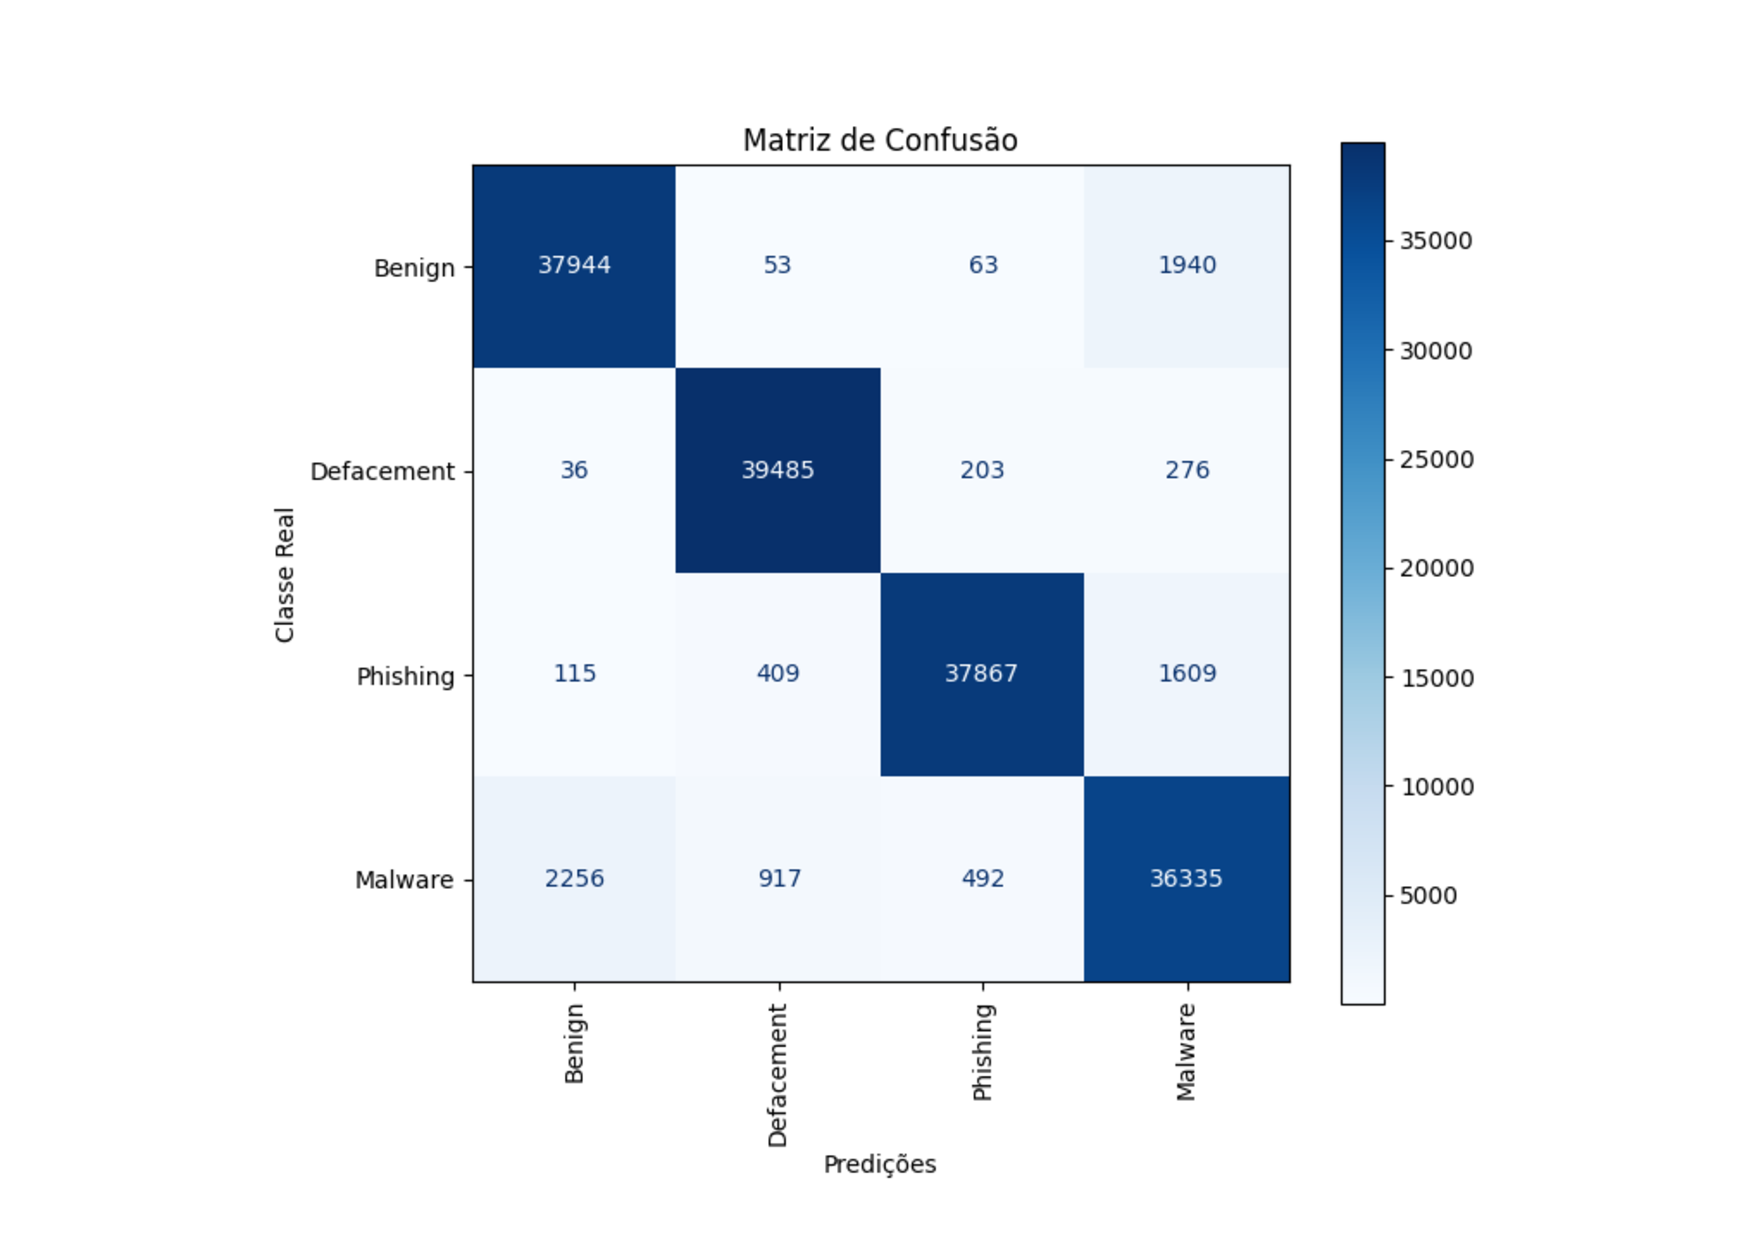
\includegraphics[width=1.1\textwidth]{pic/confusion.pdf}
    \caption{Análise de falsos negativos}
    \label{fig:exampleFig3}
\end{figure}

Como trabalhos futuros, podemos citar a necessidade de uma análise mais profunda nas características das URLs. Deve ser possível definir com mais nitidez, as linhas que delimitam os tipos de URLs maliciosas. Na Figura \ref{fig:exampleFig3}, fica evidente que ainda não existem características relevantes o suficiente para separar claramente as instâncias da classe \emph{malware} do restante das URLs. A ordem de grandeza de falsos negativos e positivos supera qualquer outro tipo de URL. Além disso, falsos negativos nesta classificação possuem potencial prejudicial descomunal, apresentando URLs de \emph{malware} como seguras.

Outro ponto que pode vir a ser explorado são os níveis de correlações entre as características. Na Figura \ref{fig:exampleFig4}, podemos observar alguns casos de forte correlação entre características. Um exemplo claro pode ser observado entre as características correspondentes ao número de diretórios e a quantidade de símbolos "/". Os valores de ambos atributos são diretamente proporcionais, logo pode-se cogitar estratégias de junção de características ou algo do gênero.

Por fim, seria interessante considerar a redução do volume da base de dados. Para isto, devemos analisar a remoção de URLs redundantes da base, ou seja, que não agregam informação útil na classificação. Aplicando a técnica de \emph{instance selection}, cria-se um potencial para redução considerável no volume dos dados, isto mantendo o desempenho dos modelos e reduzindo o custo computacional para treinamento.

\begin{figure}[H]
    \centering
    \vspace*{-1.15cm}
    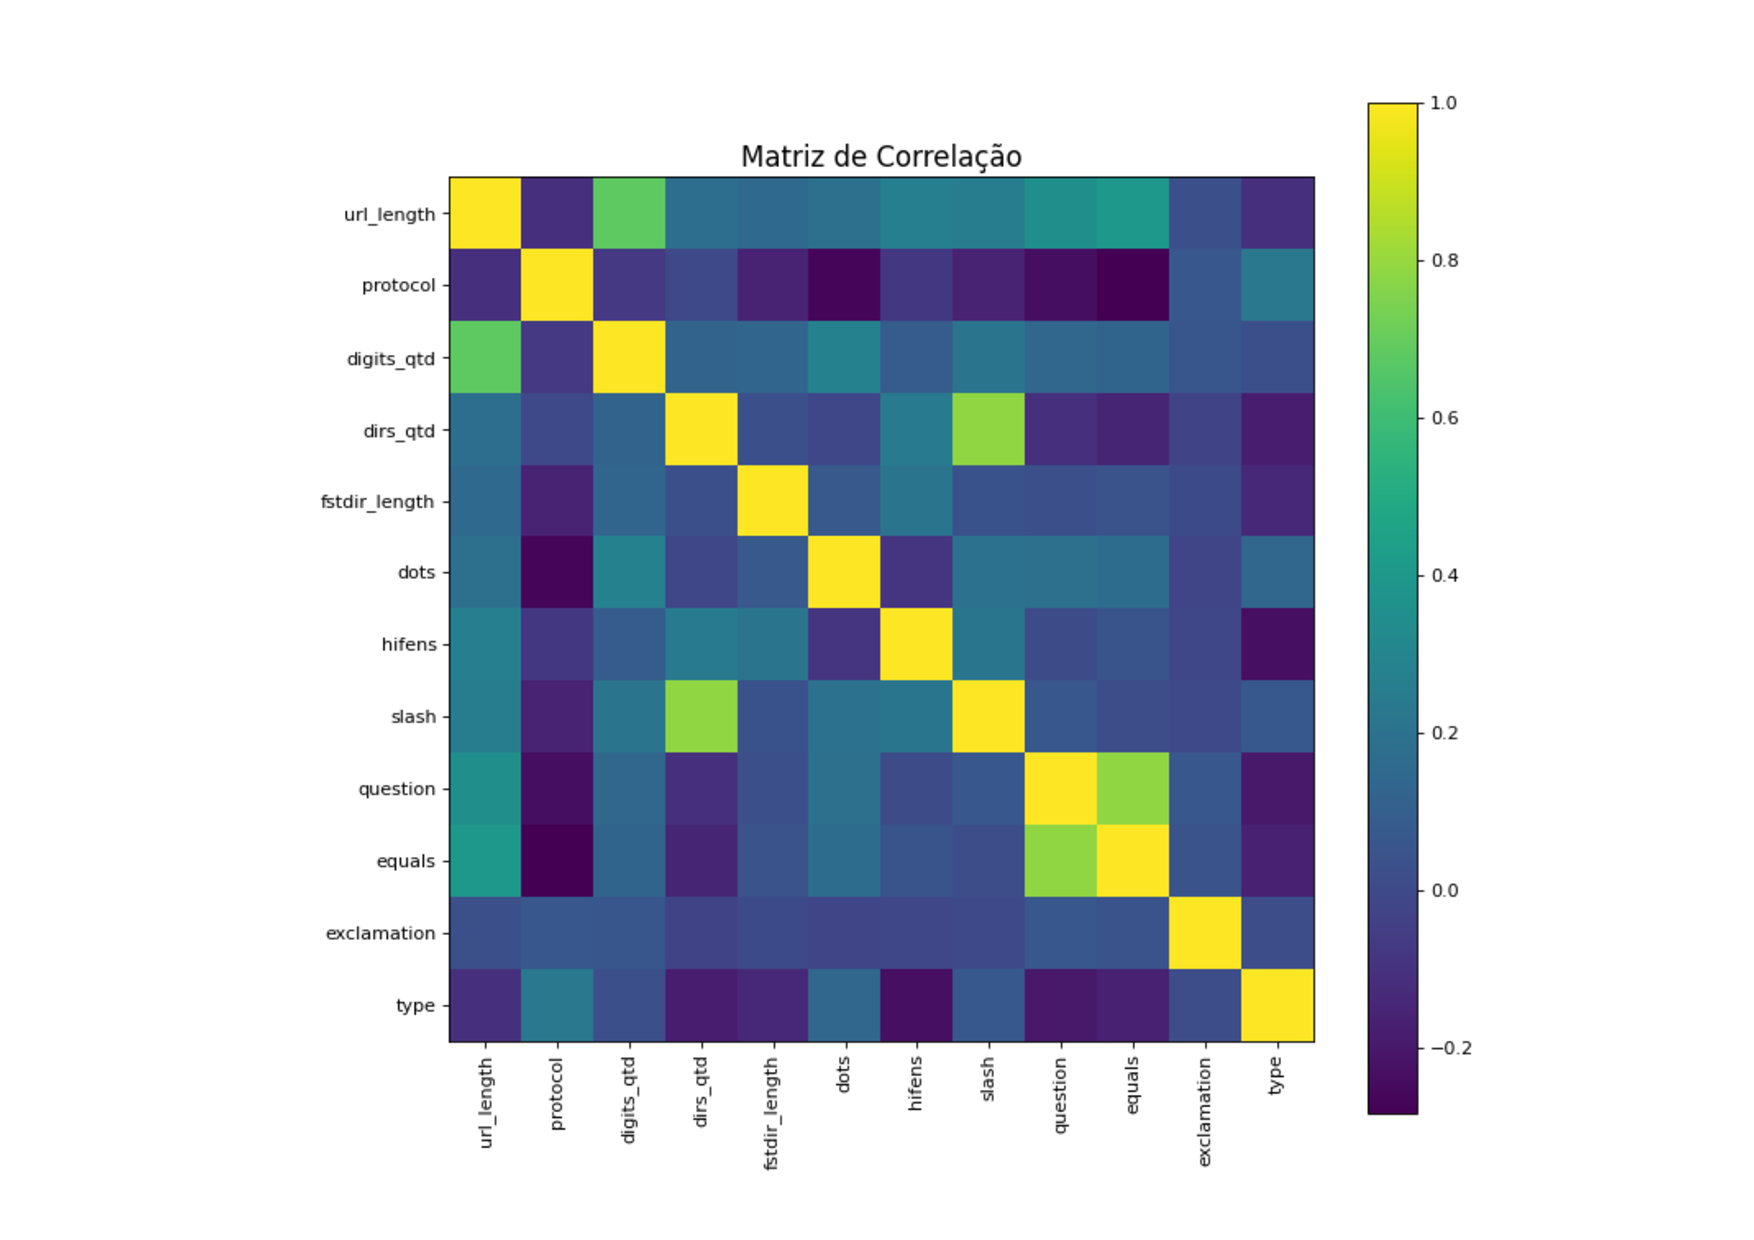
\includegraphics[width=1.1\textwidth]{pic/corr.pdf}
    \caption{Níveis de correlação entre características}
    \label{fig:exampleFig4}
\end{figure}
\vspace*{-0.5cm}

\bibliographystyle{ACM-Reference-Format}
\bibliography{sample-base}

\end{document}
